\chapter{Géométrie, information et loi de l’aire des trous noirs}

\lectureoverview{La destination annoncée est la cosmologie, mais le chemin le plus court pour y parvenir commence par un retour à la relativité restreinte. Une métrique décrit la géométrie de l’espace-temps, et la condition de temps propre nul indique comment se propage la lumière. Nous appliquerons cette règle à la géométrie de Schwarzschild, distinguerons l’horizon de la singularité, puis nous demanderons ce qu’il advient de l’information lorsqu’un trou noir rayonne et s’évapore. La réponse part de l’entropie ordinaire et aboutit à l’argument de Bekenstein fondé sur un bit : un trou noir stocke l’information par unités d’aire de l’horizon, et non de volume.}

Susskind reporte brièvement le bilan promis des succès et des échecs de la théorie des cordes. Il est tard, dit-il, et il vaut mieux parler du fond que faire un bilan. Ce soir, le fond consiste dans la géométrie et la thermodynamique minimales nécessaires pour poser le problème de l’information des trous noirs.

\section{Une règle pour la lumière}

La relativité restreinte traite l’espace et le temps comme un seul objet géométrique. Pour des événements voisins séparés par \(dt,dx,dy,dz\), Susskind adopte la convention où le signe temporel est positif et écrit
\begin{equation}
d\tau^2=dt^2-\frac{1}{c^2}\left(dx^2+dy^2+dz^2\right).
\end{equation}
Les signes opposés des termes temporel et spatial distinguent la géométrie de Minkowski de la géométrie euclidienne à quatre dimensions. Le facteur \(1/c^2\) ne sert qu’à rendre les unités compatibles ; en mesurant le temps et la distance de façon cohérente, on peut poser \(c=1\).

Pour une séparation de genre temps, \(d\tau^2>0\), et \(d\tau\) est le temps propre indiqué par une horloge qui suit la trajectoire. Les séparations de genre espace vérifient plutôt \(d\tau^2<0\). Le cas qui nous intéresse ce soir se situe exactement entre les deux. Un rayon lumineux suit une trajectoire \emph{nulle},
\begin{equation}
d\tau^2=0.
\end{equation}
En se limitant d’abord au mouvement selon l’axe \(x\), on obtient
\begin{align}
0&=dt^2-\frac{dx^2}{c^2},\\
c\,dt&=\pm dx,\\
\frac{dx}{dt}&=\pm c.
\end{align}
Les signes décrivent les rayons qui se propagent vers la droite et vers la gauche. La valeur numérique attribuée à \(c\) change lorsqu’on remplace les centimètres par des mètres ou des kilomètres ; l’énoncé invariant n’est pas un nombre, mais la condition de nullité.

En relativité générale, c’est la métrique qui se complique, pas cette règle. Avec les coordonnées \(x^\mu\), \(\mu=0,1,2,3\),
\begin{equation}
ds^2=g_{\mu\nu}(x)\,dx^\mu dx^\nu,
\end{equation}
où les indices répétés sont sommés et où les coefficients peuvent varier d’un point à l’autre. Pour trouver les directions localement accessibles à la lumière, on annule cette forme quadratique.

\section{Coordonnées sphériques et métrique de Schwarzschild}

Un trou noir non rotatif est à symétrie sphérique ; les coordonnées cartésiennes en masquent donc la structure utile. Soit \(r\) la distance radiale et \(\theta,\phi\) les coordonnées d’une direction sur une sphère unité. Son élément de ligne est
\begin{equation}
d\Omega^2=d\theta^2+\sin^2\theta\,d\phi^2.
\end{equation}
Sur une sphère de rayon \(r\), les déplacements angulaires contribuent donc par \(r^2d\Omega^2\). L’espace-temps plat en coordonnées sphériques s’écrit
\begin{equation}
d\tau^2=dt^2-\left(dr^2+r^2d\Omega^2\right),
\qquad (c=1).
\end{equation}

Susskind ne dérive pas la solution du trou noir à partir des équations d’Einstein. Il l’écrit et nous invite à l’examiner. Le tableau rend explicite la comparaison recherchée.

\begin{figure}[htbp]
\centering
\includegraphics[width=0.86\textwidth]{lecture_02_figure_02.png}
\caption{L’espace-temps plat en coordonnées sphériques, au-dessus de la déformation de Schwarzschild. Le facteur répété \(1-2GM/(c^2r)=1-R_s/r\) et le schéma radial apparaissent ensemble.}
\lectureframe{00:19:12.520}
\end{figure}

Pour un trou noir de masse \(M\), définissons le rayon de Schwarzschild
\begin{equation}
R_s=\frac{2GM}{c^2}.
\end{equation}
L’élément de ligne extérieur est
\begin{equation}
d\tau^2=\left(1-\frac{R_s}{r}\right)dt^2
-\frac{dr^2/c^2}{1-R_s/r}
-\frac{r^2}{c^2}d\Omega^2.
\label{eq:schwarzschild-explicit-c}
\end{equation}
De manière équivalente, en posant \(c=1\),
\begin{equation}
ds^2=\left(1-\frac{2GM}{r}\right)dt^2
-\frac{dr^2}{1-2GM/r}-r^2d\Omega^2.
\label{eq:schwarzschild}
\end{equation}
Loin du trou noir, \(R_s/r\ll1\), et l’on retrouve la métrique sphérique plate. Cette vérification asymptotique importe davantage que de mémoriser la formule, même si Susskind recommande cette dernière comme sujet de conversation lors des cocktails.

\editorialnote{Le tableau alterne entre \(d\tau^2\) et \(ds^2\), et n’affiche pas toujours de manière cohérente tous les facteurs de \(c\). L’équation~\eqref{eq:schwarzschild-explicit-c} suit la convention de la conférence pour la coordonnée temporelle, dans laquelle \(t\) a la dimension d’un temps. La forme standard avec \(x^0=ct\) lui est algébriquement équivalente.}

\subsection{L’horizon n’est pas la singularité}

Dans ces coordonnées, deux rayons semblent suspects. En \(r=R_s=2GM\), en unités naturelles, le coefficient de \(dt^2\) s’annule et celui de \(dr^2\) diverge. En \(r=0\), la courbure elle-même devient singulière. Il ne s’agit pas de deux versions d’un même événement :
\begin{equation}
\begin{aligned}
r=R_s &:\quad \text{horizon},\\
r=0 &:\quad \text{curvature singularity}.
\end{aligned}
\end{equation}

Les forces de marée permettent de distinguer physiquement les deux cas. Un champ gravitationnel varie d’un point à l’autre d’un corps étendu : les pieds peuvent être attirés plus fortement que la tête, ce qui étire le corps tandis que les directions transversales sont comprimées. À l’horizon, ces forces de marée restent finies ; à l’horizon d’un trou noir suffisamment massif, elles peuvent être très faibles. Rien de catastrophique ne doit nécessairement s’y produire localement. En revanche, en \(r=0\), les forces de marée divergent. Les coefficients inquiétants en \(r=R_s\) signalent un défaut des coordonnées de Schwarzschild ; la singularité en \(r=0\) est physique.

\editorialnote{On peut vérifier que la courbure reste finie en \(r=R_s\) à l’aide du scalaire de Kretschmann \(R_{\mu\nu\rho\sigma}R^{\mu\nu\rho\sigma}=48G^2M^2/(c^4r^6)\), qui est fini à l’horizon et ne diverge que lorsque \(r\to0\). Cet invariant n’a pas été écrit pendant la conférence, mais il précise la distinction entre les forces de marée.}

\section{La lumière radiale près de l’horizon}

Revenons maintenant à notre règle. Un rayon radial conserve sa position angulaire, donc \(d\Omega=0\), et un rayon lumineux vérifie \(ds^2=0\). En unités où \(c=1\), l’équation~\eqref{eq:schwarzschild} donne
\begin{equation}
0=\left(1-\frac{2GM}{r}\right)dt^2
-\frac{dr^2}{1-2GM/r}.
\end{equation}
En multipliant par \(1-2GM/r\) et en prenant la racine carrée, on obtient deux branches,
\begin{align}
dr&=\pm\left(1-\frac{2GM}{r}\right)dt,\\
\frac{dr}{dt}&=\pm\left(1-\frac{2GM}{r}\right).
\label{eq:radial-null}
\end{align}
Le signe plus correspond à la propagation vers l’extérieur, le signe moins à la propagation vers l’intérieur. Loin du trou noir, leurs vitesses coordonnées tendent vers \(\pm1\). À l’horizon, les deux vérifient \(\lvert dr/dt\rvert\to0\) : en temps coordonné de Schwarzschild, un rayon sortant semble s’y immobiliser, tandis qu’un rayon entrant met un temps coordonné infini à l’atteindre.

\begin{figure}[htbp]
\centering
\includegraphics[width=0.82\textwidth]{lecture_02_figure_03.png}
\caption{Schéma complété au tableau en coordonnées \(t\)-\(r\) : les rayons nuls radiaux deviennent presque verticaux à mesure qu’ils approchent de l’horizon en pointillés.}
\lectureframe{00:30:25.000}
\end{figure}

\begin{figure}[htbp]
\centering
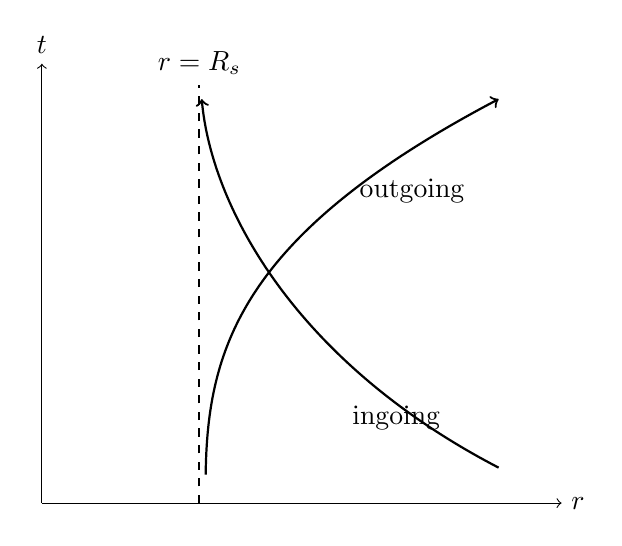
\begin{tikzpicture}[x=1.0cm,y=0.9cm]
\draw[->] (0,0) -- (6.6,0) node[right] {$r$};
\draw[->] (0,0) -- (0,6.2) node[above] {$t$};
\draw[dashed,thick] (2.0,0) -- (2.0,5.9) node[above] {$r=R_s$};
\draw[thick,->] (2.08,.4) .. controls (2.10,2.2) and (2.55,3.8) .. (5.8,5.7);
\draw[thick,->] (5.8,.5) .. controls (3.2,2.0) and (2.15,4.2) .. (2.03,5.7);
\node[align=center] at (4.7,4.4) {outgoing};
\node[align=center] at (4.5,1.2) {ingoing};
\end{tikzpicture}
\caption{Version épurée du schéma au tableau en temps coordonné. Le ralentissement apparent concerne \(t\) de Schwarzschild, et non un défaut local de propagation de la lumière à \(c\).}
\end{figure}

À l’intérieur de l’horizon, les cônes de lumière futurs s’inclinent si fortement vers l’intérieur que les deux branches radiales orientées vers le futur conduisent à des valeurs décroissantes de \(r\). Aucun signal émis depuis cette région ne peut s’échapper vers l’extérieur, et toute trajectoire causale orientée vers le futur atteint la singularité.

\begin{classroomqa}
\audiencequestion{Si la vitesse de la lumière est invariante, que signifie exactement l’affirmation selon laquelle la lumière ralentit près de l’horizon ?\lecturetimestamp{00:31:44}}
\lecturerresponse{La quantité affichée est \(dr/dt\) dans un système de coordonnées particulier. La valeur numérique d’une vitesse change déjà lorsqu’on remplace les mètres par des centimètres ; ici, les étalons radiaux et temporels effectifs varient selon la position. L’énoncé universel est que tout rayon lumineux suit une trajectoire nulle, \(ds^2=0\).}
\end{classroomqa}
\editorialnote{Un observateur local en chute libre mesure la vitesse de la lumière dans le vide comme étant \(c\) ; la vitesse nulle en coordonnées de Schwarzschild à l’horizon n’est pas une grandeur observable localement.}

\begin{classroomqa}
\audiencequestion{La même affirmation sur la vitesse nulle vaut-elle quel que soit le milieu matériel dans lequel la lumière se propage ?\lecturetimestamp{00:33:24}}
\lecturerresponse{Non. La reconnaissance disponible ne conserve pas d’explication plus détaillée de cette réponse.}
\end{classroomqa}
\editorialnote{L’affirmation concernant la vitesse de la lumière nulle porte sur sa propagation dans l’espace-temps vide. Les interactions avec la matière peuvent donner à un paquet d’ondes une vitesse effective plus faible ; c’est une propriété du milieu, pas une modification de la vitesse causale locale \(c\).}

\begin{classroomqa}
\audiencequestion{À quoi ressemble un rayon lumineux entrant sur le même diagramme \(t\)-\(r\) ?\lecturetimestamp{00:33:32}}
\lecturerresponse{C’est la branche qui semble suivre le trajet inverse : partant d’une grande valeur de \(r\), elle se courbe vers l’horizon et s’en approche asymptotiquement. Il lui faut un temps coordonné infini \(t\) pour l’atteindre.}
\end{classroomqa}
\editorialnote{Un observateur en chute libre atteint et franchit l’horizon en un temps propre fini ; seul \(t\) de Schwarzschild diverge.}

\section{Pourquoi l’évaporation pose un problème}

L’horizon mérite une étude bien plus approfondie : comment il se forme, ce que voit un observateur en chute libre, et si quelque chose d’inhabituel s’y produit localement. Susskind remet ces questions à plus tard et passe à la mécanique quantique. Du point de vue extérieur, la matière et toutes les informations qui permettent de la distinguer se trouvent comprimées toujours plus près de l’horizon et deviennent inaccessibles. Cela seul n’implique pas nécessairement une destruction de l’information ; elle peut simplement être cachée.

Le résultat de Hawking rend le problème aigu. Un trou noir classique qui a atteint un état stationnaire semble être l’objet le plus terne qui soit : sphérique, sombre et incapable d’envoyer un message. Mais ``noir'' a deux sens. Le mot peut signifier qu’il n’émet rien, ou qu’il émet un rayonnement thermique de corps noir. Un trou noir quantique est noir dans ce second sens. Il a une température, brille et perd de l’énergie. Puisque
\begin{equation}
E=Mc^2,
\qquad
R_s=\frac{2GM}{c^2},
\end{equation}
le rayonnement diminue à la fois sa masse et le rayon de son horizon. Si l’évaporation finit par faire disparaître le trou noir, qu’advient-il de l’information qui semblait rester à son horizon ? Elle pourrait être détruite, piégée dans un minuscule résidu, ou encodée dans le rayonnement sortant. La tension entre ces possibilités constitue le problème de l’information, et la théorie des cordes nous aidera plus tard à en préciser la résolution.

Ce soir, aucun calcul de théorie quantique des champs en espace-temps courbe n’est entrepris. Susskind suit plutôt la voie plus simple de Bekenstein : d’abord comprendre l’entropie comme une information, puis calculer quelle quantité d’information un trou noir peut dissimuler.

\section{Une information présente, mais cachée}

Imaginons qu’on divise une boîte en cellules suffisamment petites pour que chacune soit occupée ou vide. Une chaîne binaire---une réponse par cellule---distingue cette configuration de toutes les autres configurations permises. Pour décrire la matière de façon plus réaliste, il faut aussi poser des questions sur les espèces de particules et d’autres degrés de liberté, mais le principe reste le même : l’information se mesure par le nombre minimal de questions oui--non nécessaires pour spécifier l’état.

\begin{classroomqa}
\audiencequestion{S’agit-il uniquement d’une description d’un système statique ?\lecturetimestamp{00:45:49}}
\lecturerresponse{C’est une description instantanée, à un instant donné. La dynamique transforme ensuite cet état en un autre état.}
\end{classroomqa}

Le principe suivant est plus profond : l’évolution d’un système fermé ne fusionne pas deux états microscopiques distincts en un seul. Si deux configurations diffèrent maintenant, leurs configurations après évolution restent distinguables en principe. L’évolution hamiltonienne classique est inversible et l’évolution quantique est unitaire.\editorialnote{Les équations effectives dissipatives ne peuvent effacer des distinctions que parce que les degrés de liberté de l’environnement, qui ne sont pas observés, ont été omis ; l’état complet du système fermé les conserve.}

La baignoire rend concrète la différence entre perte et inaccessibilité. Deux suites de gouttes pourraient coder deux textes distincts en code Morse. Une fois l’eau au repos, les deux baignoires semblent identiques. Les ondulations visibles ont disparu, mais une mesure microscopique complète révélerait encore des configurations moléculaires différentes. Le message s’est dispersé parmi des degrés de liberté trop petits et trop nombreux pour être suivis.

L’entropie correspond à cette information cachée. Au regard des questions macroscopiques que nous pouvons poser---température, énergie totale, composition, niveau de l’eau---, de nombreuses distinctions microscopiques restent possibles mais inaccessibles. Dans le décompte des bits utilisé pendant la conférence,
\begin{equation}
S=\hbox{number of hidden bits}.
\end{equation}
La formule statistique précise est \(S=k_B\ln\Omega\), mais la définition qualitative suffit pour l’argument sur les trous noirs.

\section{La température, coût de la dissimulation d’un bit}

La température est facile à mesurer, mais sa définition est étonnamment indirecte. Susskind prend l’entropie et l’énergie comme concepts fondamentaux. Supposons qu’un ordinateur réinitialise un bit à une valeur standard. Le dispositif physique subsiste, mais la distinction entre ses états antérieurs zéro et un disparaît de l’ordinateur. Elle ne peut disparaître du monde physique complet ; elle est transférée à des degrés de liberté microscopiques de l’environnement, qui s’échauffe légèrement. C’est le principe de Landauer.

Si une unité d’entropie correspond à un bit et que la température se mesure en unités d’énergie, la conférence écrit
\begin{align}
\Delta S&=1,\\
\Delta E&=T\,\Delta S,\\
dE&=T\,dS.
\label{eq:first-law}
\end{align}

\begin{figure}[htbp]
\centering
\includegraphics[width=0.84\textwidth]{lecture_02_figure_04.png}
\caption{La thermodynamique de l’information au tableau : \(S\) est l’entropie, un bit caché correspond à \(\Delta S=1\) et son coût énergétique minimal s’écrit \(\Delta E=T\Delta S\).}
\lectureframe{00:58:40.000}
\end{figure}

\editorialnote{En unités conventionnelles, le coût réversible d’effacement d’un bit binaire est \(k_BT\ln2\). L’équation~\eqref{eq:first-law} utilise \(k_B=1\) et traite l’unité d’entropie de la conférence comme un bit, tout en omettant le facteur \(\ln2\) correspondant. Ces conventions n’affectent pas l’argument d’échelle qui suit.}

Selon l’estimation avancée par une personne dans le public, la hausse minimale de température provoquée par l’effacement d’environ \(100\) gigaoctets dans un verre d’eau est proche de \(10^{-15}\) degrés. Susskind retient l’idée plutôt que le nombre exact : à température ambiante, l’énergie minimale associée à un bit est extraordinairement faible, et les ordinateurs réels dissipent beaucoup plus d’énergie parce que l’effacement n’est pas réversible.

\begin{classroomqa}
\audiencequestion{L’exemple du disque dur n’est-il qu’une analogie, ou l’échauffement dû à l’effacement est-il une véritable loi ?\lecturetimestamp{01:00:02}}
\lecturerresponse{C’est une véritable contrainte physique, la règle de Landauer. La réinitialisation d’une cellule mémoire élimine de l’ordinateur l’ancienne distinction ; l’information doit donc être transférée à l’environnement. Les opérations ordinaires sont bien moins efficaces que le minimum idéal, car elles actionnent aussi les circuits, déplacent des charges et produisent de la chaleur sans rapport avec l’effacement.}
\end{classroomqa}

\begin{classroomqa}
\audiencequestion{Dissimuler un bit coûte-t-il plus d’énergie à température plus élevée ?\lecturetimestamp{01:02:07}}
\lecturerresponse{Oui. La relation \(dE=T\,dS\) l’indique précisément : pour un même transfert d’entropie, un bain thermique plus chaud exige un transfert d’énergie plus important. On peut tout aussi bien considérer cette relation entre énergie et bit caché comme une définition de la température.}
\end{classroomqa}

\begin{classroomqa}
\audiencequestion{Si l’on réécrit un bit déjà mémorisé, l’ancienne information est-elle perdue ?\lecturetimestamp{01:02:43}}
\lecturerresponse{Elle a quitté l’ordinateur, mais elle n’a pas disparu du système physique fermé. La distinction écrasée s’est dispersée dans l’environnement, où elle contribue à l’information inaccessible et donc à l’entropie.}
\end{classroomqa}

L’identification de l’entropie thermodynamique à l’information microscopique manquante remonte à Boltzmann ; au vingtième siècle, Shannon a introduit le langage correspondant de la théorie de l’information. Susskind remarque que cette explication était curieusement absente des cours de thermodynamique qu’il a suivis, comme ceux de plusieurs personnes dans le public, dans les années 1950. L’informatique a rendu le lien plus difficile à ignorer, mais n’est pas à l’origine de son contenu physique.

\section{Introduire un bit dans un trou noir}

Nous pouvons maintenant concevoir la formation d’un trou noir bit par bit, tout comme on remplit une baignoire goutte à goutte. La question est différentielle : de combien l’horizon grandit-il lorsqu’un bit supplémentaire est caché ? Commençons par un trou noir de masse \(M\) et de rayon \(R_s\), puis faisons tomber le plus simple des objets, dont la seule distinction récupérable est de savoir s’il a été absorbé.

\begin{classroomqa}
\audiencequestion{L’information ne met-elle pas un temps coordonné infini à entrer dans le trou noir ?\lecturetimestamp{01:08:07}}
\lecturerresponse{Elle est comprimée de façon exponentielle près de l’horizon et devient inaccessible à l’extérieur en un temps pratique court, même si le temps coordonné de Schwarzschild attribue une durée infinie au franchissement lui-même. Pour le bilan extérieur, on peut donc la considérer comme stockée à l’horizon.}
\end{classroomqa}

Un photon est un candidat naturel, mais un photon quelconque transporte plus d’un bit. Sa polarisation peut coder un choix binaire. Un point d’arrivée bien localisé fournit de nombreuses autres questions oui--non : hémisphère supérieur ou inférieur, moitié gauche ou droite, et ainsi de suite. La mécanique quantique limite la localisation à une longueur d’onde environ ; pour supprimer l’information de position, il faut donc utiliser la plus grande longueur d’onde que le trou noir puisse encore absorber.

\begin{classroomqa}
\audiencequestion{Existe-t-il vraiment une longueur d’onde maximale au-delà de laquelle le photon ne peut pas entrer ?\lecturetimestamp{01:12:15}}
\lecturerresponse{Oui. Une onde beaucoup plus grande que le trou noir est principalement diffusée au lieu d’être absorbée. Le choix marginal utile consiste à prendre une longueur d’onde comparable au rayon de l’horizon : assez grande pour effacer le point d’entrée, mais assez petite pour avoir une probabilité d’absorption substantielle.}
\end{classroomqa}

\begin{classroomqa}
\audiencequestion{La direction d’arrivée du photon apporte-t-elle elle-même de l’information ?\lecturetimestamp{01:13:28}}
\lecturerresponse{Pour une longueur d’onde de l’ordre de la taille de tout l’horizon, le champ varie si lentement à travers le trou noir que la direction d’arrivée ne peut être résolue avec précision. C’est pourquoi la limite des grandes longueurs d’onde se ramène à une seule donnée oui--non, plutôt qu’à un impact précisément localisé.}
\end{classroomqa}

On choisit donc, à l’ordre de grandeur près,
\begin{equation}
\lambda\sim R_s=\frac{2GM}{c^2}.
\label{eq:one-bit-wave}
\end{equation}
La cinématique du photon donne
\begin{equation}
E=cp,
\qquad
p=\hbar k=\frac{h}{\lambda},
\qquad
\Delta E\sim\frac{\hbar c}{R_s}.
\label{eq:one-bit-energy}
\end{equation}
Ici, \(k=2\pi/\lambda\) et \(h=2\pi\hbar\). La conférence néglige délibérément le facteur \(2\pi\), ainsi que les facteurs d’absorption d’ordre unité.

\begin{classroomqa}
\audiencequestion{Faut-il écrire la quantité de mouvement \(\hbar/\lambda\) ou \(h/\lambda\) ?\lecturetimestamp{01:16:00}}
\lecturerresponse{Avec \(\lambda\) comme longueur d’onde ordinaire, la relation exacte est \(p=h/\lambda=2\pi\hbar/\lambda\) ; avec le nombre d’onde \(k=2\pi/\lambda\), elle est \(p=\hbar k\). Dans cette estimation, on ne conserve que l’échelle ; le facteur \(2\pi\) est donc délibérément omis.}
\end{classroomqa}

Le coût énergétique pour cacher un bit est fixé par l’échelle de température. Les équations~\eqref{eq:one-bit-wave} et~\eqref{eq:one-bit-energy} donnent donc
\begin{equation}
k_BT_H\sim\frac{\hbar c}{R_s}
\sim\frac{\hbar c^3}{GM}.
\end{equation}
Le résultat exact de Hawking est
\begin{equation}
k_BT_H=\frac{\hbar c^3}{8\pi GM}.
\end{equation}
L’argument élémentaire retrouve la dépendance en \(M,G,c,\hbar\), mais pas le coefficient.

\section{Un bit occupe une cellule à l’échelle de Planck}

Le même photon nous indique de combien l’horizon grandit. Son énergie modifie la masse de
\begin{equation}
\Delta M=\frac{\Delta E}{c^2}
\sim\frac{\hbar}{cR_s}.
\end{equation}
Puisque \(R_s=2GM/c^2\),
\begin{equation}
\Delta R_s=\frac{2G}{c^2}\Delta M
\sim\frac{G\hbar}{c^3R_s},
\end{equation}
où tous les facteurs d’ordre unité ont de nouveau été omis. En multipliant par \(R_s\),
\begin{equation}
R_s\Delta R_s\sim\frac{G\hbar}{c^3}.
\end{equation}
Comme \(A=4\pi R_s^2\), sa différentielle est \(dA=8\pi R_s\,dR_s\). Par conséquent,
\begin{equation}
\Delta A\sim\frac{G\hbar}{c^3}=\ell_P^2,
\qquad
\ell_P=\sqrt{\frac{G\hbar}{c^3}}.
\label{eq:planck-patch}
\end{equation}

\begin{figure}[htbp]
\centering
\includegraphics[width=0.84\textwidth]{lecture_02_figure_05.png}
\caption{L’argument d’échelle complété au tableau : l’énergie \(\Delta E\sim\hbar c/R_s\) nécessaire pour un bit entraîne une variation de l’ordre de \(G\hbar/c^3\) pour le carré du rayon, et donc pour l’aire.}
\lectureframe{01:22:40.000}
\end{figure}

Pendant le calcul en direct, les facteurs de \(c\) sont réintroduits à mi-parcours et une personne dans le public remarque l’absence de \(c^{-2}\) dans le rayon de Schwarzschild. Cette correction est précisément ce qui fait apparaître le facteur \(c^{-3}\) dans l’équation~\eqref{eq:planck-patch}.

\begin{classroomqa}
\audiencequestion{Le fait de n’avoir réintroduit \(c\) que dans une partie du calcul a-t-il fait perdre deux puissances de ce facteur ?\lecturetimestamp{01:21:18}}
\lecturerresponse{Oui. La relation dimensionnelle est \(R_s=2GM/c^2\), et non simplement \(2GM\). La réintroduction de ce facteur donne à l’aire l’échelle \(G\hbar/c^3\).}
\end{classroomqa}

En utilisant \(G\simeq6.7\times10^{-11}\,\mathrm{m^3\,kg^{-1}\,s^{-2}}\), \(\hbar\simeq1.05\times10^{-34}\,\mathrm{J\,s}\) et \(c^3\simeq2.7\times10^{25}\,\mathrm{m^3\,s^{-3}}\),
\begin{equation}
\ell_P^2\simeq2.6\times10^{-70}\,\mathrm{m^2},
\qquad
\ell_P\simeq1.6\times10^{-35}\,\mathrm{m}.
\end{equation}
Pendant l’estimation au tableau, les puissances prononcées au fil de la conférence varient ; la conclusion physique, elle, reste stable. Cette échelle est très inférieure à ce qui est directement mesurable expérimentalement.

L’image marquante est celle de bits impénétrables, aux coudes pointus, qui s’accumulent sur l’horizon en se poussant les uns les autres. Chaque nouveau bit occupe environ une cellule de Planck. C’est une métaphore du décompte de l’aire, et non l’affirmation que des carreaux littéraux composent l’horizon.

\begin{classroomqa}
\audiencequestion{Si le premier photon est encore en approche lorsqu’un autre photon agrandit l’horizon, le premier ne se retrouve-t-il pas à l’intérieur du nouvel horizon ?\lecturetimestamp{01:26:39}}
\lecturerresponse{Cette représentation statique simplifiée ne permet pas de trancher la question avec précision. Dans un espace-temps dynamique, l’horizon des événements doit être défini globalement, et sa position change lorsque de la matière arrive. Dans la description extérieure utilisée ici, l’information reste associée à l’horizon qui grandit. La définition rigoureuse de cet horizon est reportée à plus tard.}
\end{classroomqa}

\begin{classroomqa}
\audiencequestion{Le même problème se poserait-il si l’on ajoutait une masse énorme, par exemple lors de la collision de deux trous noirs ?\lecturetimestamp{01:27:03}}
\lecturerresponse{Oui ; dans ce cas, il est impossible d’ignorer le caractère dynamique. La conférence reporte l’étude complète de la géométrie de la fusion jusqu’à ce que l’horizon ait été défini plus précisément.}
\end{classroomqa}

\begin{classroomqa}
\audiencequestion{L’aire de Planck est-elle définie uniquement sur une portion plane, et non sur un horizon sphérique ?\lecturetimestamp{01:27:30}}
\lecturerresponse{C’est une échelle d’aire sur une surface sphérique, et non une exigence de planéité de l’horizon. Pour ce décompte, la distinction entre plan et sphère n’a pas d’importance.}
\end{classroomqa}
\editorialnote{Lorsque le rayon de courbure de l’horizon est énorme par rapport à \(\ell_P\), chaque voisinage de taille de Planck est presque plat localement.}

Pour un trou noir de huit kilomètres de diamètre, le photon marginal correspondant est une onde radio de grande longueur d’onde, de cette échelle environ. Une analogie proposée par une personne dans le public compare la variation d’aire indépendante de la taille à l’ajout d’une même longueur de circonférence à une corde enroulée autour d’un ballon de basket ou de la Terre : dans les deux cas, l’écart radial ainsi créé est le même. Les géométries exactes diffèrent, mais les deux exemples isolent une variation indépendante de la taille initiale de l’objet.

\section{La loi de l’aire}

L’ajout de bits un à un modifie l’aire de l’horizon d’une même quantité microscopique universelle. Le nombre de bits pouvant être cachés doit donc être proportionnel à \(A/\ell_P^2\), et non au volume. Bekenstein a déduit cette proportionnalité ; le calcul de Hawking en a fixé le coefficient :
\begin{equation}
S_{\mathrm{BH}}=\frac{k_B A c^3}{4G\hbar}
=\frac{k_B A}{4\ell_P^2}.
\label{eq:bh-entropy}
\end{equation}
Si l’entropie est comptée en bits binaires plutôt qu’en unités thermodynamiques, il faut diviser \(S_{\mathrm{BH}}/k_B\) par \(\ln2\).

\begin{figure}[htbp]
\centering
\includegraphics[width=0.84\textwidth]{lecture_02_figure_06.png}
\caption{La formule finale au tableau, avec le facteur de Hawking \(1/4\) : \(S\propto Ac^3/(4G\hbar)\) dans les unités d’entropie de la conférence.}
\lectureframe{01:31:02.000}
\end{figure}

Les trous noirs ont donc beaucoup plus d’entropie que les systèmes ordinaires de taille comparable, et ce de façon considérable. Pourtant, le résultat reste inférieur à ce que laisserait penser un décompte naïf en volume. L’information indépendante est bornée par une grandeur de surface. Cette inversion---une région gravitationnelle tridimensionnelle décrite par une information qui évolue comme une frontière bidimensionnelle---est à l’origine du principe holographique.

\begin{classroomqa}
\audiencequestion{D’où vient le facteur \(1/4\) dans la formule de l’entropie ?\lecturetimestamp{01:30:30}}
\lecturerresponse{L’argument de Bekenstein fixait la dépendance en l’aire et les constantes fondamentales, mais laissait le coefficient indéterminé ; ses estimations donnaient des possibilités telles que des logarithmes de deux. Le calcul de théorie quantique des champs de Hawking a fixé le coefficient à \(1/4\) exactement.}
\end{classroomqa}

La position de \(\hbar\) réserve la dernière surprise. On pourrait s’attendre à ce qu’une entropie quantique soit proportionnelle à \(\hbar\) et s’annule dans la limite classique. Or \(\hbar\) se trouve au dénominateur. Lorsque \(\hbar\to0\), une onde peut porter une information arbitrairement fine à un coût énergétique arbitrairement faible ; la capacité d’entropie diverge donc. La quantification n’ajoute pas une entropie infime à un trou noir autrement classique ; elle empêche que la capacité d’information soit infinie.

\begin{classroomqa}
\audiencequestion{Pourquoi \(\hbar\), dont la dimension est celle du moment cinétique, fixe-t-il aussi la relation entre la quantité de mouvement ordinaire et la longueur d’onde ?\lecturetimestamp{01:33:23}}
\lecturerresponse{\(\hbar\) a la dimension d’une action, soit celle d’une quantité de mouvement multipliée par une distance. Puisque \(p\lambda\) a cette même dimension, la relation quantique peut s’écrire \(p\sim\hbar/\lambda\), à un facteur \(2\pi\) près, selon la convention choisie. Le moment cinétique \(\mathbf r\times\mathbf p\) a la même dimension pour la même raison.}
\end{classroomqa}

La conférence s’arrête ici, non parce que le sujet est épuisé, mais parce qu’il s’agit du bon point d’arrêt. La géométrie nous a expliqué pourquoi l’horizon dissimule l’information ; la thermodynamique nous a appris à compter l’information cachée ; la mécanique quantique a fourni une aire finie par bit. La question suivante n’est plus de savoir si un trou noir possède des états microscopiques, mais comment ces états encodent ce qui est tombé dedans et le restituent finalement.
